% Archivo: sections/4_results_and_discussion.tex

\section{Resultados y Discusión}

\subsection{Dinámica Multivariable y Transición al Caos}

Las Figuras \ref{fig:dynamics_cte} y \ref{fig:dynamics_no_cte} presentan el análisis exhaustivo de la cinemática, la topología del espacio de fases, y las métricas de estabilidad para diferentes regímenes del sistema. En particular, en la Figura \ref{fig:dynamics_cte} se varía exclusivamente el ángulo inicial, mientras que en la Figura \ref{fig:dynamics_no_cte} se varía tanto el ángulo inicial como el coeficiente de amortiguamiento.

\begin{figure}[h]
    \centering
    \includegraphics[width=1\textwidth]{figures_tex/chaos_q_cte.png}
    \caption{Paneles dinámicos multivariables ($\theta_0^{(1)} = 11.46^\circ, \ \theta_0^{(2)} = 11.56^\circ, \, q^{(1)}=q^{(2)} = 0.5 $). De izquierda a derecha: Serie temporal $\theta(t)$, Espacio de fases $(\theta, \omega)$, Sección de Poincaré, Evolución del exponente de Lyapunov ($\lambda$), y Espectro de potencia en frecuencia.}
    \label{fig:dynamics_cte}
\end{figure}


\begin{itemize}
        \item \textbf{Régimen Periódico ($F_D = 0.50,\ 0.95$):} Las series temporales $\theta(t)$ son regulares. El espacio de fases muestra ciclos límite cerrados, obviando la fase transitoria. Las secciones de Poincaré se reducen a puntos discretos. El exponente de Lyapunov converge a valores negativos ($\lambda < 0$). El espectro de potencia presenta picos discretos bien definidos correspondientes a la frecuencia de forzamiento y sus armónicos. Nótese que, al no apreciarse variación significante entre un ángulo inicial y otro, las curvas se solapan observándose exclusivamente las líneas verdes correspondientes al segundo elemento graficado.
        \item \textbf{Régimen Caótico ($F_D = 1.20$):} La serie temporal pierde periodicidad. El espacio de fases se vuelve denso y entrelazado. La sección de Poincaré muestra la formación de atractores extraños. Esto se puede ver con más claridad en la Figura \ref{fig:poincare}, cuyo diagrama en detalle revela el comportamiento fractal del atractor, observándose multiples capas finamiente espaciadas. Crucialmente, el exponente de Lyapunov se vuelve positivo ($\lambda > 0$).        
        
        \item \textbf{Re-estabilización ($F_D = 1.44, \ 4.00$):} El sistema recupera la regularidad, mostrando nuevamente ciclos límite complejos pero cerrados, $\lambda < 0$ y espectros discretos.

        \item \textbf{Punto de Transición ($F_D =  1.48$):} Punto crítico donde el exponente de Lyapunov se anula ($\lambda = 0$). Este valor marca la transición de la cascada de duplicación de periodo hacia un régimen aperiódico, como se observa en la Figura \ref{fig:bifurcacion}.
        
\end{itemize}

\begin{figure}[h]
    \centering
    \includegraphics[width=1\textwidth]{figures_tex/chaos_q_no_cte.png}
    \caption{Paneles dinámicos multivariables ($\theta_0^{(1)} = 11.46^\circ, \ \theta_0^{(2)} = 11.56^\circ, \, q^{(1)}=0.5, \ q^{(2)} = 0.6 $). De izquierda a derecha: Serie temporal $\theta(t)$, Espacio de fases $(\theta, \omega)$, Sección de Poincaré, Evolución del exponente de Lyapunov ($\lambda$), y Espectro de potencia en frecuencia.}
    \label{fig:dynamics_no_cte}
\end{figure}

La variación del coeficiente de amortiguamiento junto con las condiciones angulares iniciales provoca que, para las distintas fuerzas $F_D$ empleadas, no se obtenga un exponente de Lyapunov negativo. Salvo en el caso $F_D = 1.22$, con $\lambda \approx 0.01$, el resto de ejemplos tienen asociados un exponente $\lambda \approx 0$. Estos valores cercanos a cero indican que el sistema se encuentra en un régimen cuasiperiódico, en el que no colapsa hacia un régimen estable ni caótico.

Por último, para poder obtener una mayor resolución en la sección de Poincaré, se resuelve el mismo sistema que en el caso de la Figura \ref{fig:dynamics_cte} para $F_D = 1.2$, pero empleando un tiempo de integración de 7000 segundos, en comparación con los 100 segundos empleados previamente. El resultado muestra la estructura fractal del atractor y se puede hallar en la Figura \ref{fig:poincare}.


Se pueden visualizar los vídeos del péndulo forzado para las distintas $F_D$ en \href{https://www.youtube.com/shorts/_VPDbxwMFOg}{YouTube}.

\begin{figure}
    \centering
    \href{https://youtube.com/playlist?list=PLYDzV8MgIoOP_vNYarRFVN29fjnX_ux3A&si=TuSaNbOAATZLORfA}{
    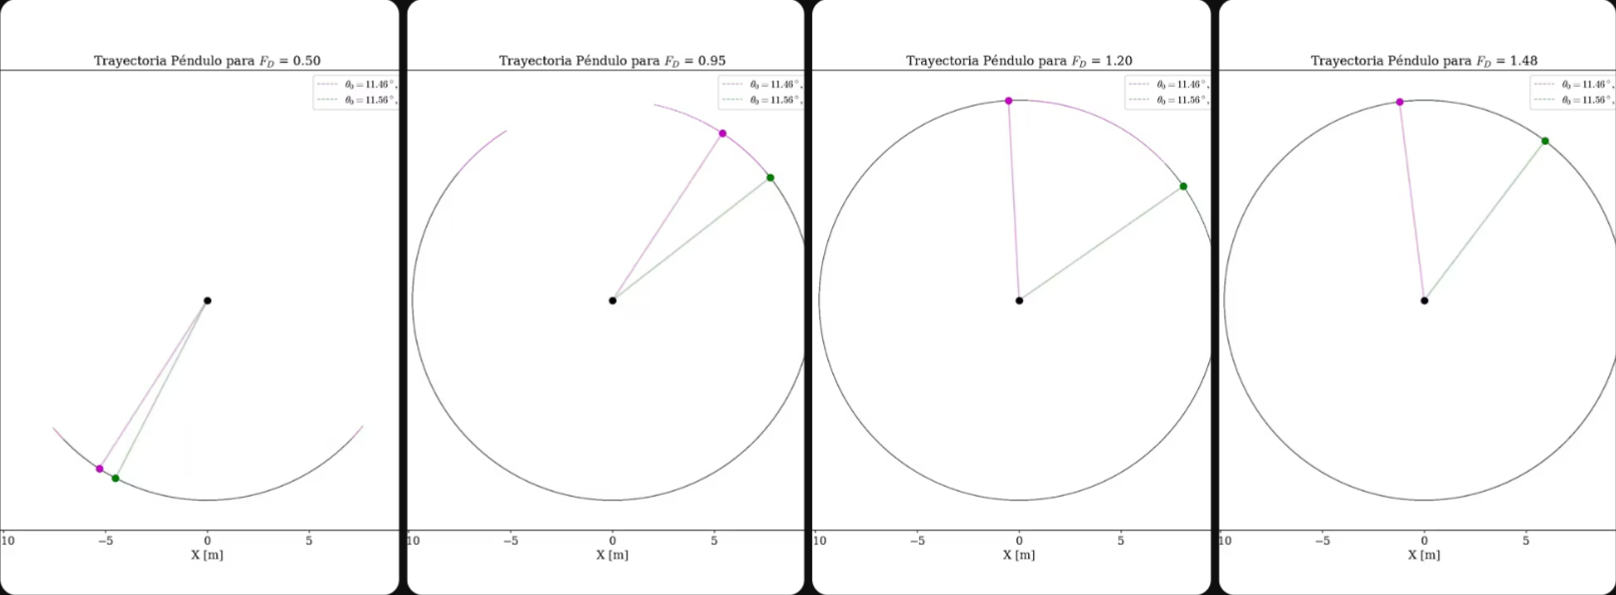
\includegraphics[width=0.5\linewidth]{figures_tex/videos.png}
    }
\end{figure}






\begin{figure}[h!]
    \centering
    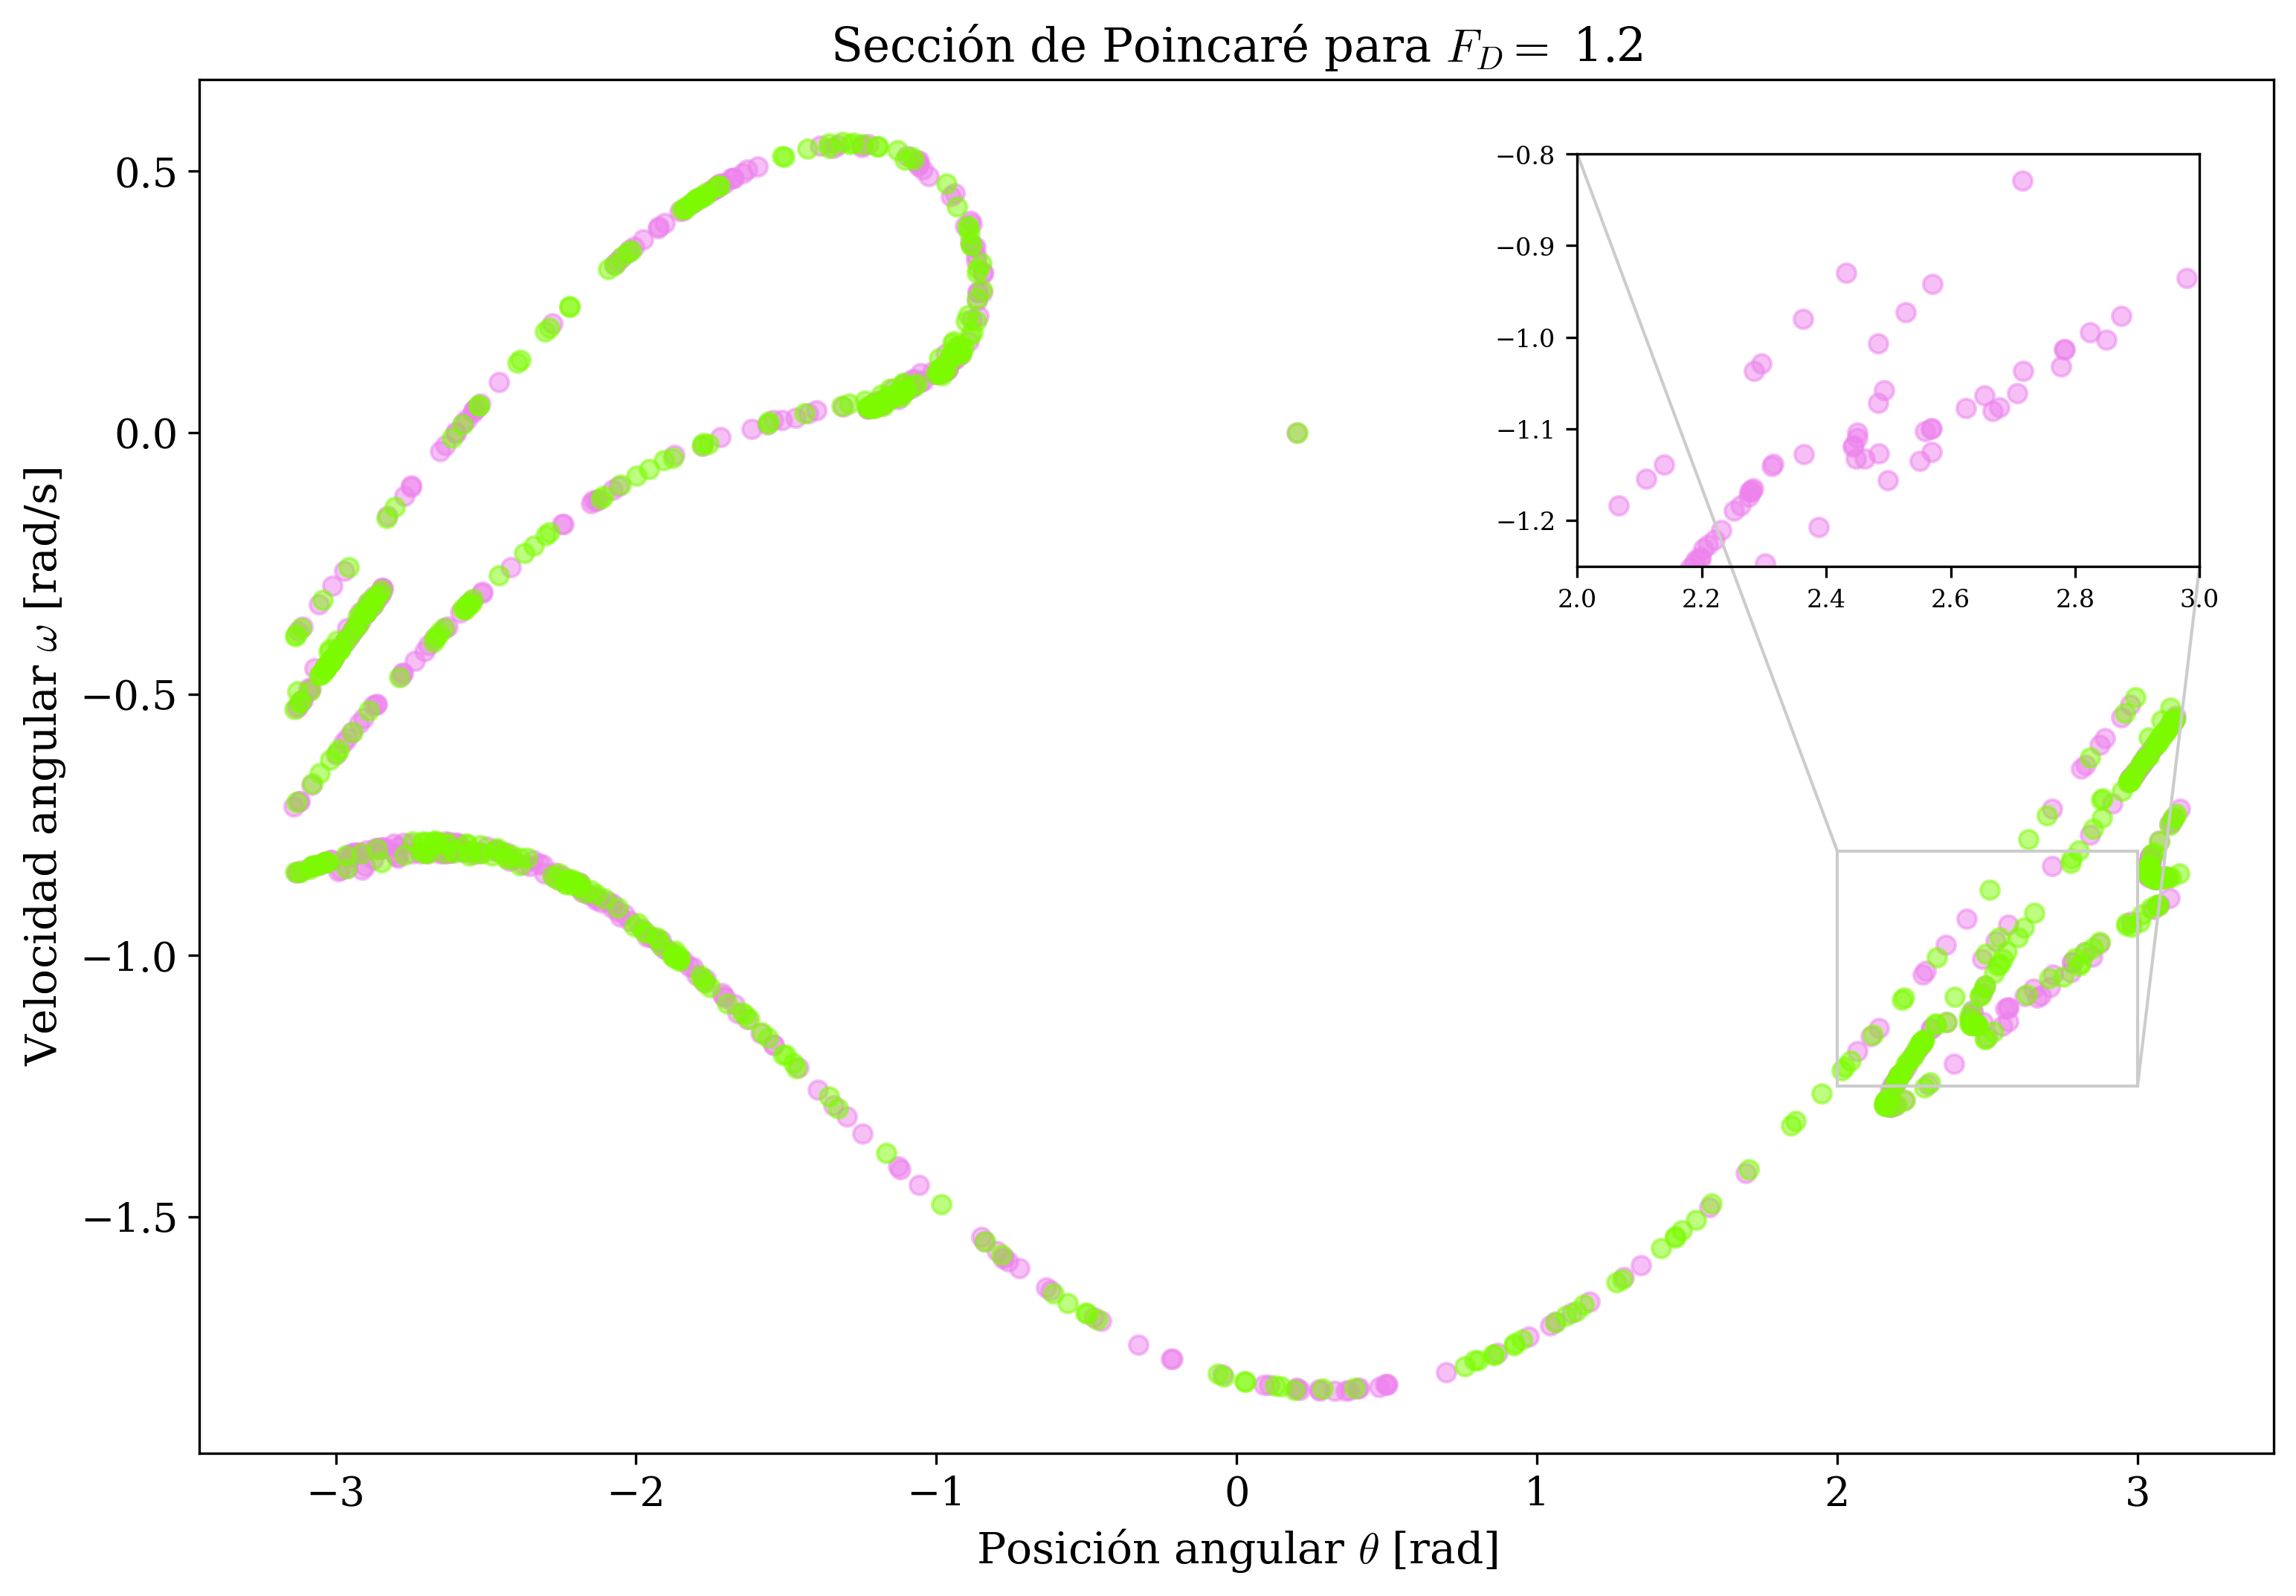
\includegraphics[width=0.8\textwidth]{figures_tex/poincare_extenso.png}
    \caption{Sección de Poincaré en el plano de fases ($\theta$, $\omega$) para una fuerza impulsora $F_D = 1.2$. El recuadro superior derecho muestra una ampliación de una región específica del atractor donde se observa el comportamiento fractal del mismo.}
    \label{fig:poincare}
\end{figure}




\subsection{Diagramas de Bifurcación}

La transición hacia el caos a medida que se incrementa la amplitud de la fuerza impulsora se observa claramente en un diagrama de bifurcación, como los de la Figura \ref{fig:bifurcacion}. En esta se muestran dicha representación tanto para el ángulo como para la velocidad angular. 

\begin{figure}[h]
    \centering
    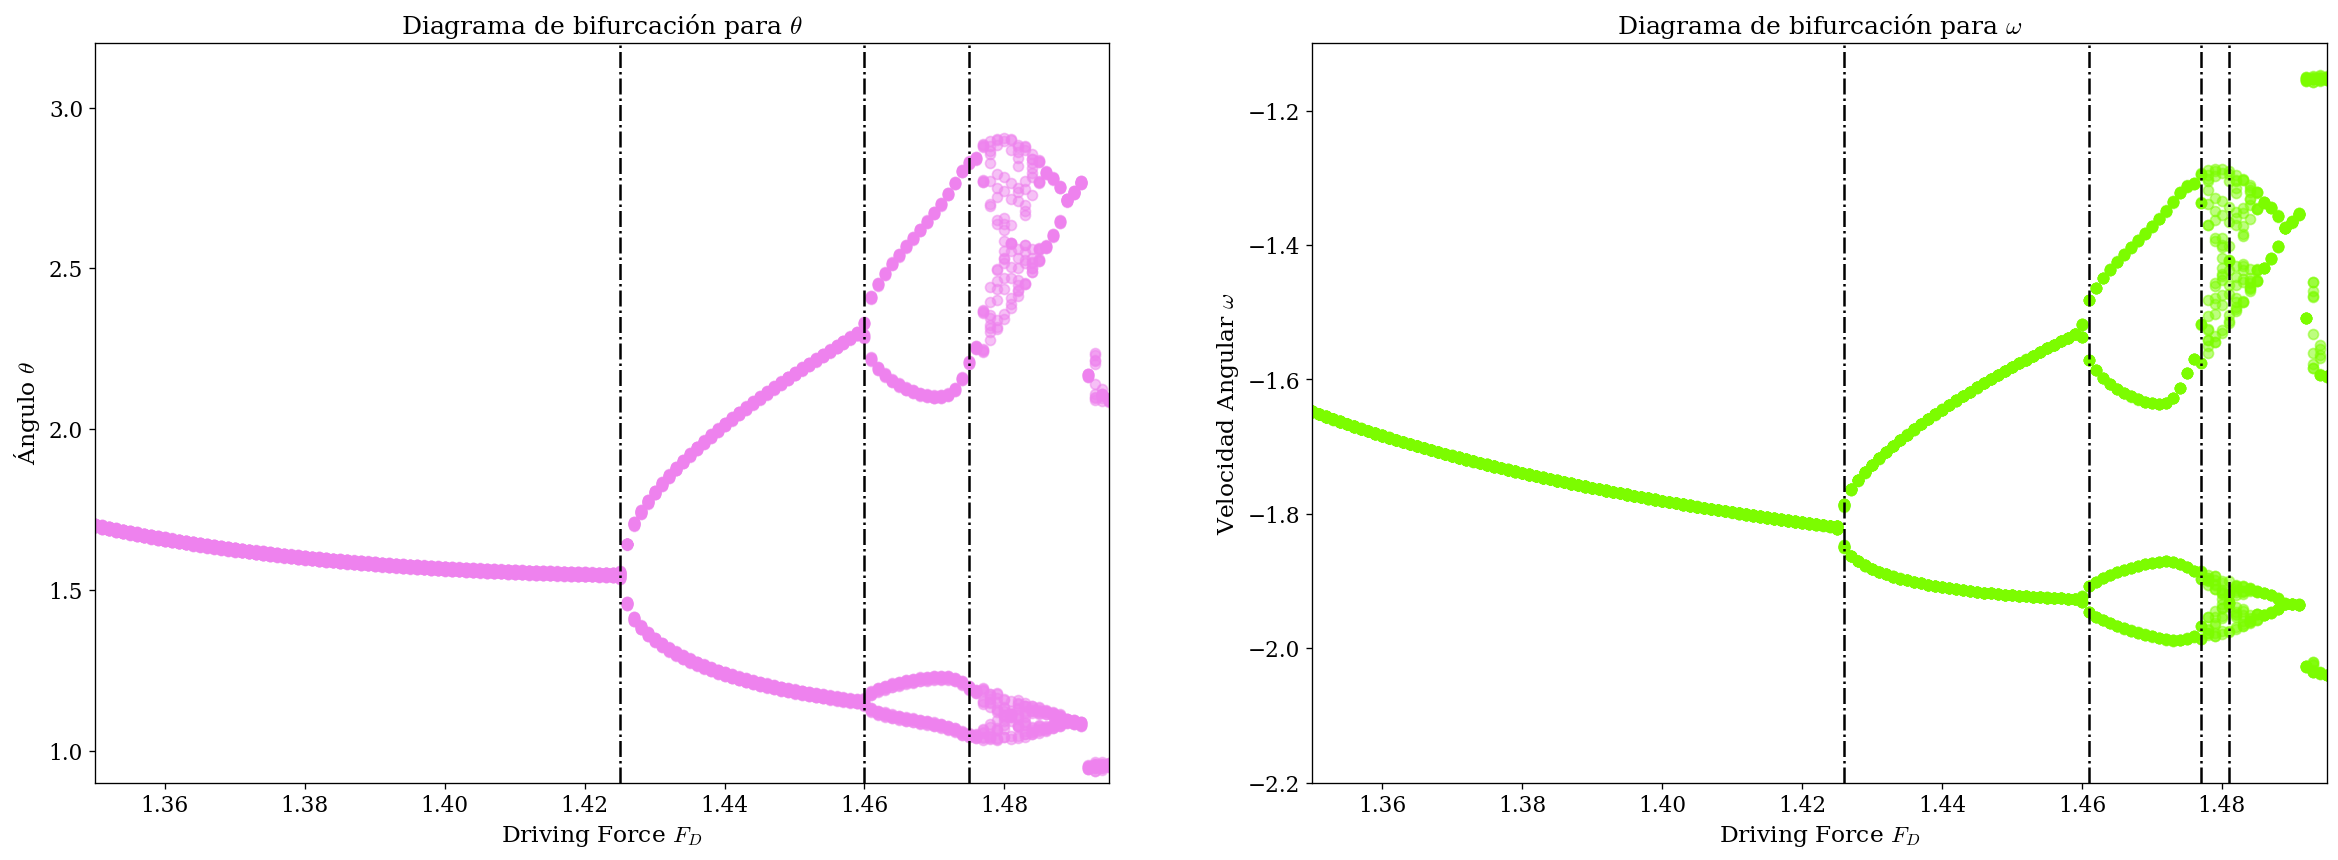
\includegraphics[width=0.9\textwidth]{figures_tex/bifurcation.png}
    \caption{Diagramas de bifurcación para la posición angular ($\theta$) y la velocidad angular ($\omega$) en función de la fuerza impulsora ($F_D$). Las líneas discontinuas marcan los puntos críticos de duplicación de periodo.}
    \label{fig:bifurcacion}
\end{figure}

    Para valores bajos de $F_D$ (e.g., $F_D < 1.42$), el sistema presenta un único atractor de periodo 1, indicando un movimiento armónico estable. En $F_D \approx 1.425$, se observa la primera bifurcación, donde el sistema oscila entre dos estados (periodo 2). Sucesivas bifurcaciones ocurren en intervalos cada vez más cortos (e.g., $F_D \approx 1.46$ para periodo 4), culminando en regiones densas que denotan comportamiento caótico ($F_D \gtrsim 1.48$).

    Este comportamiento es característico de una cascada de Feigenbaum, la cual describe una ruta clásica hacia el caos determinista a través de la duplicación de periodo. La existencia de bandas continuas en $\theta$ y $\omega$ confirma que, para ciertos valores de $F_D$, el sistema explora una infinidad de estados en el espacio de fases sin repetir su trayectoria.

    Mediante el gráfico de bifurcación se podría obtener la constante de Feigenbaum, $\delta$, sin embargo, requeriría de una resolución temporal y en el paso de barrido $\Delta F_D$ demasiado pequeñas, resultando computacionalmente costoso, por lo que queda fuera de este estudio.

\subsection{Más sistemas caóticos: Péndulo doble y Atractor de Lorenz}

En este apartado se presenta la simulación de dos sistemas caóticos, presumiblemente, los dos sistemas caóticos más famosos en el imaginario colectivo: el péndulo doble y el Atractor de Lorenz. Ambos se encuentran animados en \href{https://www.youtube.com/watch_videos?video_ids=L4-EepwR-u8,ykCy39y1Cbk}{YouTube}.


\begin{figure}[h]
    \centering
        \begin{minipage}{0.48\textwidth}
        \centering
        \href{https://youtu.be/L4-EepwR-u8}{
        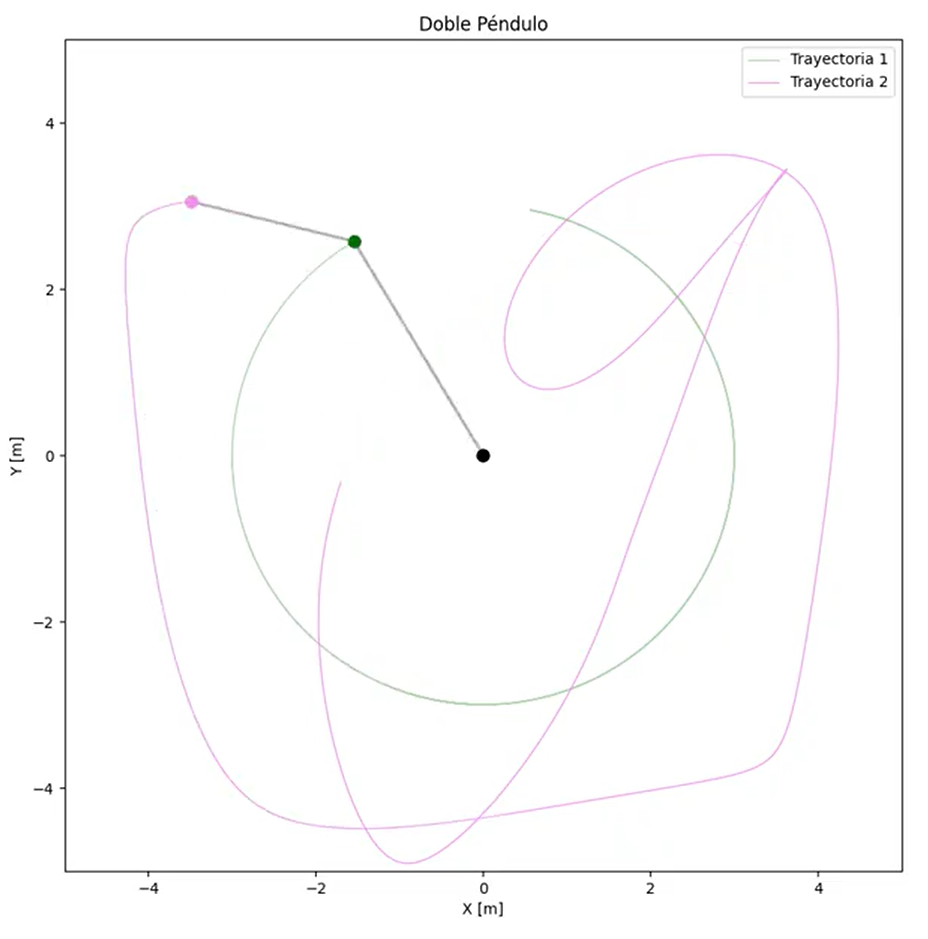
\includegraphics[width=\linewidth]{figures_tex/pend_doble.png}}
        \caption{Animación del péndulo doble.}
    \end{minipage}
    \hfill 
\begin{minipage}{0.48\textwidth}
        \centering
    \href{https://youtu.be/ykCy39y1Cbk}{
        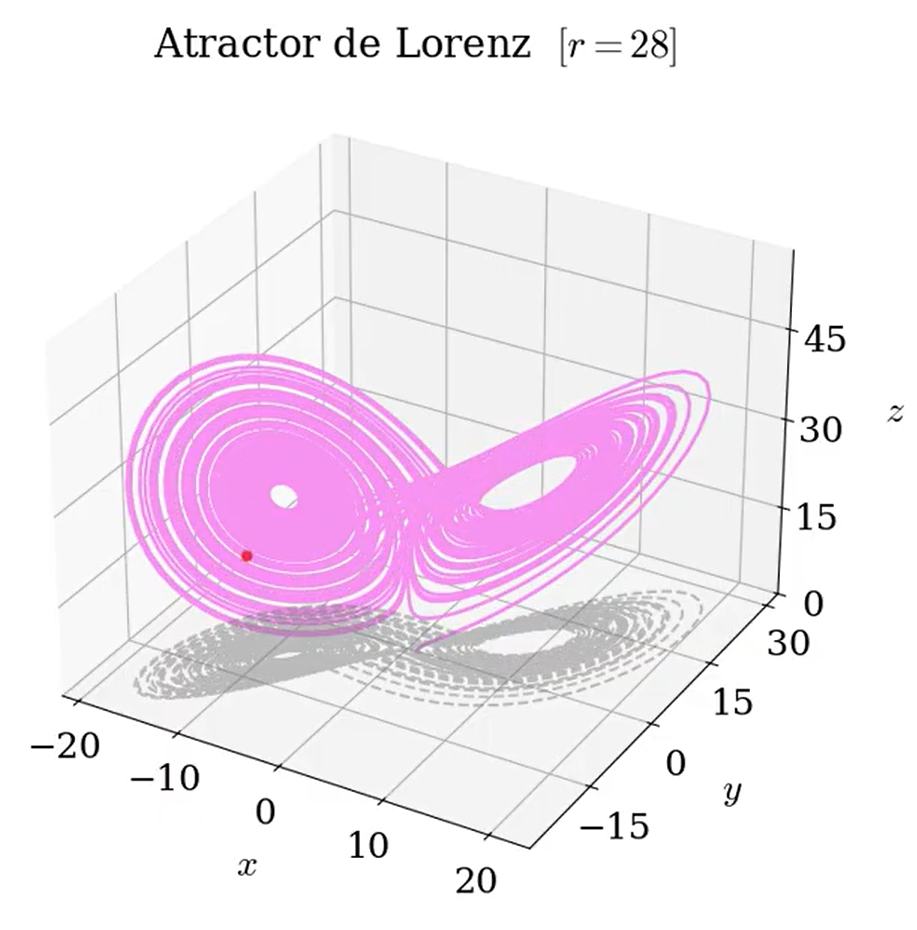
\includegraphics[width=\linewidth]{figures_tex/lorenz_atractor.png}}
        \caption{Animación del Atractor de Lorenz.}
    \end{minipage}
\end{figure}